\documentclass{article}
\usepackage{makeidx}
\usepackage{lmodern}
\usepackage{amssymb}
\usepackage[T1]{fontenc}
\usepackage[spanish,activeacute]{babel}
\usepackage[utf8]{inputenc}
\usepackage{graphicx}
\graphicspath{ {../img/} {./img/} }
\usepackage{minted}
\newtheorem{ppio}{Principio }

\begin{document}

\title{Principio de Invarianza}
\author{Carlos Sánchez Páez}
\maketitle
\newpage

\section{Introducción}
El objetivo de este ejercicio es demostrar el Principio de Invarianza mediante la ejecución de un algoritmo (concretamente el de ordenación por burbuja). Dicho principio estipula lo siguiente: 
\begin{ppio}[de Invarianza]
Dos implementaciones diferentes de un  mismo  algoritmo  no  difieren  en  eficiencia  más  que,  a  lo  sumo,  en  una constante multiplicativa.
\end{ppio}
Es decir, podemos cambiar de plataforma para que nuestro algoritmo se ejecute más rápido, pero el factor que nos proporcionará una mejora significativa con respecto al tamaño del problema será un \textbf{cambio de algoritmo}. 
\section{Código fuente empleado}
Los ficheros fuente que emplearemos para realizar el ejercicio han sido descargados de la plataforma \textit{decsai.ugr.es}. Consisten en una implementación en Java y C++ del algoritmo de ordenación de un vector utilizando el método \textbf{burbuja}. 
\newline
Cada programa crea un vector de tamaño variable en cada iteración (de 1.000 a 20.000 incrementando de 1.000 en 1.000) ordenado de forma decreciente. Tras ésto, aplica el método burbuja para ordenarlo, obteniendo así los tiempos del peor caso.

\begin{figure}[H]
\begin{minted}{c++}
#include <iostream>
#include <ctime>
using namespace std;

void Burbuja(double *v, int posini, int posfin) {
    int i, j;
    double aux;
    bool haycambios= true;
    i= posini;
    while (haycambios) {
        haycambios=false; // Suponemos vector ya ordenado
        // Recorremos vector de final a i
        for (j= posfin; j>i; j--) {
            // Dos elementos consecutivos mal ordenados
            if (v[j-1]>v[j]) {
                aux= v[j]; // Los intercambiamos
                v[j]= v[j-1];
                v[j-1]= aux;
                // Al intercambiar, hay cambio
                haycambios= true;
            }
        }
        i++;
	}
}

int main()
{
    const int SIZE= 20000;
    double vect[SIZE];
    unsigned long tini, tfin;
    for (int TAM= 1000; TAM<=SIZE; TAM+= 1000) {
        for (int i= 0; i<TAM; i++)
            vect[i]= TAM-i;     
        tini= clock(); // Tiempo inicial
        Burbuja(vect, 0, TAM-1);
        tfin= clock(); // Tiempo final
        cout<<"N: "<<TAM<<" T (ms.): "<<1000.0*(tfin-tini)/(double)CLOCKS_PER_SEC<<endl;
    }
    return 0;
}
\end{minted}
\caption{Código en C++}
\end{figure}

\begin{figure}[H]
\begin{minted}{java}
public class BurbujaJava {
    public static void Burbuja (double [] v, int posini, int posfin) {
        int i, j;
        double aux;
        boolean haycambios= true;
        i= posini;
        while (haycambios) {
            haycambios=false; // Suponemos vector ya ordenado
            // Recorremos vector de final a i
            for (j= posfin; j>i; j--) {
                // Dos elementos consecutivos mal ordenados
                if (v[j-1]>v[j]) {
                    aux= v[j]; // Los intercambiamos
                    v[j]= v[j-1];
                    v[j-1]= aux;
                    // Al intercambiar, hay cambio
                    haycambios= true;
                }
            }
            i++;
        }
    }
    public static void main(String[] args) {
        final int SIZE= 20000;
        double []vect= new double[SIZE];
        long tini, tfin;
        for (int TAM= 1000; TAM<=SIZE; TAM+= 1000) {
            // Ejemplo: Vector al revés
            for (int i= 0; i<TAM; i++) 
                vect[i]= TAM-i;
            tini= System.currentTimeMillis(); // Tiempo inicial
            Burbuja(vect, 0, TAM-1);
            tfin= System.currentTimeMillis(); // Tiempo final
            System.out.println("N: "+TAM+" T (ms): "+(tfin-tini));
        }
    }  
}
\end{minted}
\caption{Código en Java}
\end{figure}
\section{Metodología}
Para realizar el ejercicio, programaremos un pequeño archivo \textit{makefile} con las opciones básicas, como compilar el código fuente y ejecutarlo exportando la salida a un archivo de texto, compilar la memoria y limpiar los archivos residuales y resultados.
\begin{figure}[H]
\begin{minted}{makefile}

#Definimos etiquetas
DOC=doc
SRC=src
OUTPUTFOLDER=output
CPPNAME=BurbujaC
JAVANAME=BurbujaJava
CPPOUTPUT=cpp.out
JAVAOUTPUT=java.out

#Compilar el archivo C++
all : ejecutar

cpp :
	g++ -o $(SRC)/$(CPPNAME) $(SRC)/$(CPPNAME).cpp

#Compilar el archivo Java

java : 
	javac $(SRC)/$(JAVANAME).java

#Ejecutamos cada uno y guardamos en la salida

ejecutar : cpp java
		cd $(SRC);./$(CPPNAME) > ../$(OUTPUTFOLDER)/$(CPPOUTPUT)
		cd $(SRC);java $(JAVANAME) > ../$(OUTPUTFOLDER)/$(JAVAOUTPUT)
#LaTEX

memoria : 
	pdflatex -shell-escape -synctex=1 -interaction=nonstopmode $(DOC)/memoria.tex 

#Limpiar

clean :
	rm -f $(SRC)/$(CPPNAME) $(SRC)/$(JAVANAME)

mrproper : clean
	rm -f $(OUTPUTFOLDER)/*
\end{minted}
\caption{Makefile}
\end{figure}
\section{Resultados}
Los resultados obtenidos son los siguientes:

\begin{table}[H]
\begin{center}
\begin{tabular}{|c|c|c|c|}
\hline
\textbf{Tamaño del problema} & \textbf{C++} & \textbf{Java} & \textbf{Constante multiplicativa} \\
\hline \hline
1000 & 3.247 & 8.000 & 0.0406 \\ 
\hline
2000 & 14.841 & 4.000 & 3.710 \\
\hline
3000 & 34.166 & 8.000 & 4.271 \\
\hline
4000 & 67.824 & 13.000 & 5.217 \\
\hline
5000 & 111.634 & 20.000 & 5.582 \\
\hline
6000 & 136.076 & 29.000 & 4.692 \\
\hline
7000 & 182.814 & 40.000 & 4.570 \\
\hline
9000  &	326,151  & 66,000  & 4,942 \\
\hline
10000 &	413,116  & 82,000  & 5,038 \\
\hline
11000 &	511,706  & 99,000  & 5,169 \\
\hline
12000 &	592,085	 & 117,000 & 5,061 \\
\hline
13000 &	671,105	 & 137,000 & 4,899 \\
\hline
14000 &	803,409	 & 160,000 & 5,021 \\
\hline
15000 &	896,108  & 183,000 & 4,897 \\
\hline
16000 &	983,140	 & 208,000 & 4,727 \\
\hline
17000 &	1110,460 & 235,000 & 4,725 \\
\hline
18000 &	1257,570 & 264,000 & 4,764 \\
\hline
19000 &	1385,760 & 293,000 & 4,730 \\
\hline
20000 &	1553,040 & 326,000 & 4,764 \\
\hline
\textbf{Media} & 270.705 & 63.789 & \textbf{4.244} \\
\hline
\end{tabular}
\caption{Tiempos obtenidos y constante multiplicativa.}
\end{center}
\end{table}
\section{Conclusiones}
Tras hacer las correspondientes pruebas, vemos que el algoritmo ejecutado en Java es mucho más rápido que el de C++, aproximadamente:
\[
tiempo_{java} = \frac{tiempo_{c++}}{4.244} \rightarrow tiempo_{c++} = 4.244 \cdot tiempo_{java}
\]
Es decir, si ejecutamos la ordenación mediante burbuja en Java obtendremos un rendimiento más de cuatro veces superior al que obtendríamos en C++.
\newline
Con ésto queda demostrado el Principio de Invarianza, ya que se cumple que:
\begin{figure}[H]
\begin{equation}
t_1(n) \leq t_2(n) \rightarrow \exists c \in \mathbb{R} : t_2(n) = c \cdot t_1(n)
\end{equation}
\caption{Consecuencia del Principio de Invarianza}
\end{figure}
\newpage
\section{Gráficas}
\begin{figure}[H]
   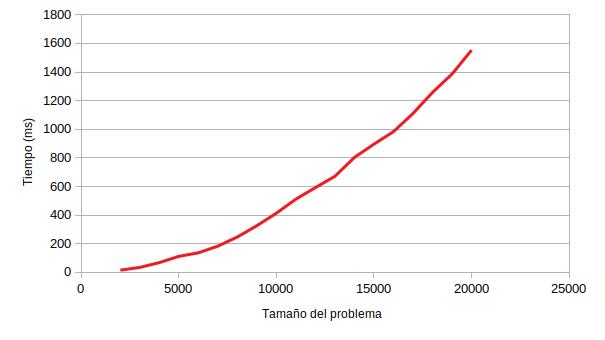
\includegraphics[width=1\textwidth]{tiempos_cpp.jpg}
  \caption{Ejecución del algoritmo en C++}
\end{figure}
\begin{figure}[H]
 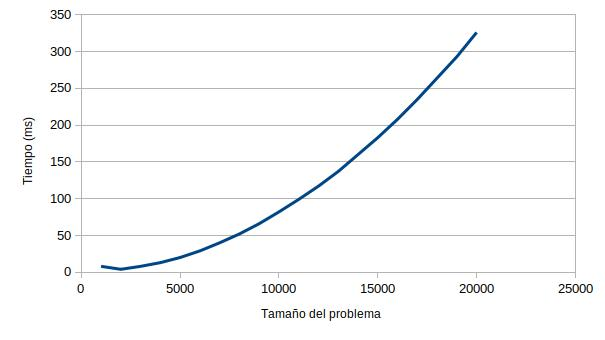
\includegraphics[width=1\textwidth]{tiempos_java.jpg}
  \caption{Ejecución del algoritmo en Java}
\end{figure}
\end{document}